% --------------------------------------------------------------------------- %
% !TEX encoding = UTF-8 Unicode
% !TEX TS-program = pdflatex
% !TEX root = main.tex
% !TEX spellcheck = en-EN
% --------------------------------------------------------------------------- %

\chapter{Review of Falling-Snow Models}
	In this chapter the theoretical framework behind a general drag coefficient model will be explained and a review of the available models in literature will be proposed. 
	
	Recalling from \sref{sec: NonSphericalParticles}, the formula used for these models is the following:
	\begin{equation}
		c_D = c_D(Re, \text{model}, \text{parameters})
	\end{equation}
	
	The main physical quantities used in this definition will now be clarified, referring the reader to the nomenclature for a comprehensive list of the names of the other variables and the terms appearing in the equations.
	The drag coefficient is defined as:
	\begin{equation}
		c_D = \dfrac{F_D}{\frac{1}{2} \rho u^2 S_{\perp}}
	\end{equation}
	with $ F_D $ being the drag force, $ \rho $ being the fluid density, and $ S_{\perp} $ being the projection of the area of the particle on a plane normal to the velocity vector ($ \underline{u} $).
	
	The models provide a constitutive relation for the drag coefficient, using non-dimensional parameters such as the Reynolds Number ($ Re $) and other quantities describing the shape of the particle and its orientation.
	 
	The characteristic dimension of the particle ($ \dv $), which appears in the definition of the Reynolds Number and the drag coefficient ($ c_D $), is defined as the diameter of the volume-equivalent sphere. Furthermore, the Reynolds number of the particle is based on the relative velocity of the fluid w.r.t. the particle:
	\begin{equation}
		Re = \dfrac{u \ \dv}{\nu} \qquad \text{with: } \qquad u := || \underline{u}_f - \underline{u}_p ||
	\end{equation}

	The parameter mainly used to describe the shape of the particle is the \textit{sphericity}, which is the ratio between the surface area of the
	volume-equivalent sphere and the area of the actual particle:
	\begin{equation}
		\Phi = \dfrac{\pi \ \dv^2} {A_{\textup{p}}}
	\end{equation}
	This is a common element between various models. The choice of the parameter that describes the particle orientation is more ample, thus each one of those parameters will be presented in relation with the linked model.
	
	\section{Chhabra review}
		In 1999 Chhabra et al. published a review article on non-spherical particles \cite{ChhabraEtAl-1999}. They evaluated a selection of the most used correlations methods using experimental results culled from 19 independent studies, consisting of 1900 data points with wide ranges of physical and kinematics conditions as: sphericity ranging from $ 0.09 $ to $ 1 $ and the Reynolds number ranging from $ 10^{-4} $ to $  5 \cdot 10^{5} $. The performances of the methods were evaluated by calculating the mean and maximum error with respect to a certain shape category (sphere, cube, cylinder and so on) and considering the overall data set. 
		The best method appeared to be that of Ganser \cite{Ganser-1993} which will be discussed in the following section.
		Yet, a more significant contribution of this article was the definition
		of a new standard for a non-spherical particle model, stating that a good correlation formula must account for information on 2 main aspects: \textit{shape} of the particle (sphericity) and \textit{orientation} of the particle. 
		
		In the following sections the Ganser model, alongside with a more recent one, will be reviewed and compared on the basis of the available literature. 
		
	\section{Ganser - 1993}
		The Ganser model \cite{Ganser-1993} comes from empirical correlations of the general drag formula by Haider and Levenspiel \cite{HaiderLevenspiel-1989}:
		\begin{equation}
			c_D = \frac{24}{Re} (1 + A Re^B) + \dfrac{C}{1 + \frac{D}{Re}}
		\end{equation}
	
		It relies on the notion that a good $ c_D $ formula must involve a dependence on at least two shape descriptors. Using similarity arguments and dimensional analysis, Ganser showed that knowledge of the Stokes' shape factor ($ K_1 $) and of the Newton's shape factor ($ K_2 $) is sufficient for accurate prediction of the drag over a large range of Reynolds number. 
		Geometric shape descriptors such as sphericity are used	to model $ K_1 $ and $ K_2 $ and not $ c_D $, directly.
		
		The basic assumption in this paper is that every isolated particle experiences a Stokes’ regime where the drag is proportional to velocity and a Newton’s regime where the drag is proportional to the square of velocity. 
		
		In addition, it is possible to extract shape and orientation factors	from the behaviour of the particle in the Stokes’s and Newton’s regimes with dimensional analysis. Then, the way a particle behaves in these two regimes can be used to predict the drag for a large range of Reynolds numbers.
		
		The general definition for the Stokes' shape factor reads:
		\begin{equation}
			K_1 = \left( \frac{1}{3} \frac{\dn}{\dv} + \frac{2}{3} \Phi^{-\frac{1}{2}} \right)^{-1} -2.25 \frac{\dv}{D_{\textup{tube}}} 
		\end{equation}
		where the importance of both the shape and the orientation of the particle in the viscous regime ($ Re \ll 1 $) is measured by the \textit{sphericity} ($ \Phi $) and the ratio between the \textit{normal diameter} (diameter of the sphere with the equivalent projected area) and the \textit{volume diameter} ($ \dn / \dv $), as already claimed by Leith \cite{Leith-1987} (who first introduced the Stokes' shape factor). Physically, values of $ \dn / \dv $ greater than 1 correspond to a particle with the axis parallel to the direction of motion bigger than the other one as prolate spheroids and cylinders. Particles with $ \dn / \dv < 1 $ are, instead, more similar to oblate spheroids and disks.
		Since we will consider only snowflakes falling in an open environment, the second term is negligible, as $ D_{\textup{tube}} \rightarrow \infty $.
		
		Thompson and Clark \cite{ThompsonClark-1991} defined the Newton's shape factor as the ratio between the drag coefficient of a particle of a certain shape and the drag coefficient of a sphere, both at Reynolds number of 10 000, following the argument that, at high Reynolds (Newton's regime), the $ c_D $ is approximately constant.
		From this observation, Ganser derived the following formula for the Newton's shape factor:
		\begin{equation}
			K_2 = 10^{1.8148 (-log(\Phi))^{0.5743}}
		\end{equation}
		
		The final version of the model is function of the \textit{generalized} Reynolds number ($ Re K_1 K_2 $) and reads:
		\begin{equation}
			c_D = K_2 \left( \frac{24}{Re K_1 K_2} (1 + 0.1118 (Re K_1 K_2)^{0.6567}) + \frac{0.4305}{1 + \frac{3305}{Re K_1 K_2}}\right) 
		\end{equation}
	
				
	\section{H\"{o}lzer and Sommerfeld - (2008)}
		The model by H\"{o}ltzer and Sommerfeld \cite{HoltzerSommerfeld-2008} is, in effect, an interpolation of previous models coming from an extensive literature review. The coefficients of their final formula are tuned on a collection of over two thousand experimental data. The $ c_D $ values used are summarized in \fref{fig: LitReviewHS}, featuring spheres, disk and plates, lengthwise spheroids and streamline bodies, isometric particles such as cubes, tetrahedrons and octahedrons, and irregularly shaped particles such as minerals.
		
		\begin{figure}
			\centering
			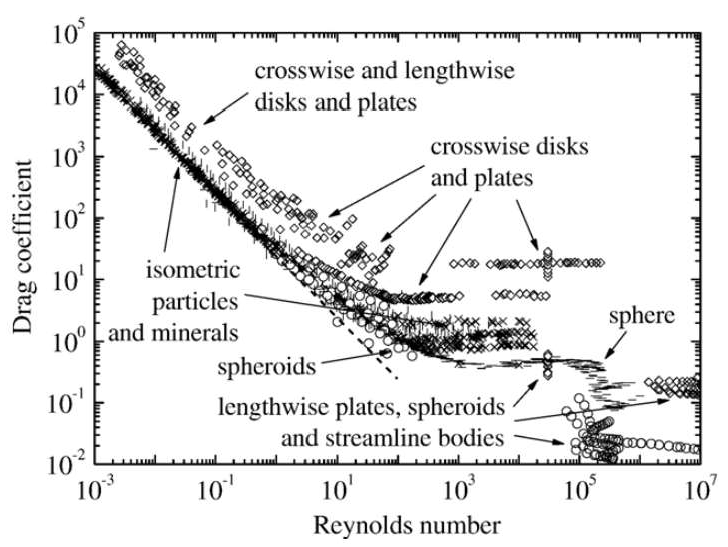
\includegraphics[width=\linewidth]{LitReviewHS.png}
			\caption[Drag coefficient of different shaped particles as function of the Reynolds number.]{Drag coefficient of different shaped particles as function of the Reynolds number. Data from the literature review of Holtzer and Sommerfeld. \cite{HoltzerSommerfeld-2008}
			Legend: $ \tikz[baseline] {\draw[dashed] (0,.7ex)--(.3,.7ex) ;} $ Stokes, 
			$ \tikz[baseline] {\draw (0,.7ex)--(.3,.7ex) ;} $ Sphere,
			$ \diamond $ Disks and plates, $ \times $ Isometric bodies, $ | $ Minerals, $ \circ $ Spheroids and streamline bodies.}
			\label{fig: LitReviewHS}
		\end{figure}

		Similarly to Ganser, they used different models for the Stokes' and the Newton's regime. The Stokes' region is characterized by an inverse proportionality between the drag coefficient and the Reynolds number. The formula used is the one suggested by Leith \cite{Leith-1987}:
		\begin{equation}
			c_D = \frac{8}{Re} \frac{1}{\sqrt{\Phi_{\perp}}} + \frac{16}{Re} \frac{1}{\Phi}
			\label{eq: Leith}
		\end{equation}
		where the particle orientation is measured by the crosswise sphericity ($ \Phi_{\perp} $), which is defined in \eref{eq: Crosswise} as the ratio between the cross-sectional area of the volume-equivalent sphere w.r.t. the cross-sectional area of the actual particle projected on a plane perpendicular to the velocity vector ($ A_{\textup{p}, \perp} $).
		\begin{equation}
			\Phi_{\perp} = \dfrac{\frac{\pi}{4}\ \dv^2} {A_{\textup{p}, \perp}}
			\label{eq: Crosswise}
		\end{equation}
		Again, to give a physical interpretation of this shape descriptor, values of $ \Phi_{\perp} $ lesser than 1 correspond to a particle with the axis parallel to the direction of motion bigger than the other one as prolate spheroids and cylinders. On the contrary, particles with $ \Phi_{\perp} > 1 $ are more similar to oblate spheroids and disks.
		The first term in \eref{eq: Leith} stands for the pressure or form drag, associated with the size of the projected cross-sectional area, while the second term represents the friction drag, associated with the size of the surface area. Correlation with experimental data showed that the use of the lengthwise sphericity ($ \Phi_{/\!/} $) instead of $ \Phi_{\perp} $ in \eref{eq: Leith} leads to a better approximation of the $ c_D $ in the Stokes region. The lengthwise sphericity is defined in \eref{eq: Lengthwise} as the ratio between the cross-sectional area of the volume-equivalent sphere and the difference between half the surface area ($ A_{\textup{p}} $) and the mean longitudinal (i.e. parallel to the direction of relative flow) projected cross-sectional area of the actual particle ($ \bar{A}_{\textup{p},/\!/} $). Since $ A_{\textup{p},/\!/} $ depends on the angle of view, an arithmetic average over an entire revolution is used.
		\begin{equation}
			\Phi_{/\!/} = \dfrac{\frac{\pi}{4}\ \dv^2} {\Delta A} \qquad \text{with: } \qquad \Delta A = \dfrac{A_{\textup{p}}}{2} - \bar{A}_{\textup{p},/\!/}
			\label{eq: Lengthwise}
		\end{equation}

		For the Newton's regime two different models are used. The first one represents the friction drag of lengthwise particles (small cross-sectional area). The mathematical model describing this phenomenon is, according to Blasius' theory:
		\begin{equation}
			c_D = 1.327 \cdot 2 \left(\frac{8}{9}\right)^{\frac{1}{4}} \pi^{\frac{1}{4}} \left(\frac{\text{depth}}{\text{length}}\right)^{\frac{1}{4}} \frac{1}{\Phi^{\frac{3}{4}}} \frac{1}{\sqrt{Re}}
			\label{eq: Blasius}
		\end{equation}
		which, for square plates, reduces to:
		\begin{equation}
			c_D = 3.43 / (\Phi^{\frac{3}{4}} \sqrt{Re})
			\label{eq: SimpleBlasius}
		\end{equation}
		and this simplified version will be used.
		
		The second model derives from the study of Tran-Cong et al \cite{TranCongEtAl-2004} and represents the behaviour of isometric and cross-wise oriented bodies. The $ c_D $ of such particles in the Newton's regime is almost solely determined by form drag, in particular it is approximately proportional to the reciprocal of crosswise sphericity. Merging this study with the literature by Ganser and Leith, H\"{o}ltzer and Sommerfeld proposed the following formula for isometric and crosswise oriented particles at high Reynolds number:
		\begin{equation}
			c_D = 0.4210^{0.4(-\log \Phi)^{0.2}} \frac{1}{\Phi_{\perp}}
			\label{eq: TranCong}
		\end{equation}

		The correlation formula for the $ c_D $ over the entire range of $ Re  $ results from the addition of Equations \ref{eq: Leith}, \ref{eq: SimpleBlasius} and \ref{eq: TranCong}:
		\begin{equation}
			c_D = \frac{8}{Re} \frac{1}{\sqrt{\Phi_{/\!/}}} 
			    + \frac{16}{Re} \frac{1}{\sqrt{\Phi}} 
			    + \frac{3}{\sqrt{Re}} \frac{1}{\Phi^{\frac{3}{4}}} 
			    + 0.4210^{0.4(-\log \Phi)^{0.2}} \frac{1}{\Phi_{\perp}}
			\label{eq: HS}
		\end{equation}
	
		In the same paper, they also derived a simplified model of similar performance, in terms of accuracy w.r.t.\ all the available data, depending on two parameters only, namely $\Phi$ and $\Phi_{\perp}$, which reads:
		\begin{equation}
			c_D = \frac{8}{Re} \frac{1}{\sqrt{\Phi_{\perp}}} 
			    + \frac{16}{Re} \frac{1}{\sqrt{\Phi}} 
			    + \frac{3}{\sqrt{Re}} \frac{1}{\Phi^{\frac{3}{4}}} 
			    + 0.4210^{0.4(-\log \Phi)^{0.2}} \frac{1}{\Phi_{\perp}}
			\label{eq: SimpleHS}
		\end{equation}
		
		During this thesis we will take advantage of the simplified model, since it reduces the number of unknowns.
		
%	\section{Heymsfield and Westbrook - (2010)}
%		Description of the model ans why it doesn't work.

	\section{Model comparison}
		Both the models presented so far have the characteristics to properly describe an arbitrary-shaped particle. Referring to the comparison done by H\"{o}lzer and Sommerfeld \cite{HoltzerSommerfeld-2008}, the Ganser formula works better with isometric particle, having a mean relative deviation of 6.46\%, over the one of 10.9\% of \eref{eq: SimpleHS}. These statistics come from the comparison of the $ c_D $ expected by the model w.r.t. the one found in the literature, considering 655 experimental data. Using the same type of comparison they found that their model has an edge on the calculation of the $ c_D $ of disk and plates (386 values), with a mean deviation of 16.8\% over the $ 1.8 \cdot 10^3 \% $ of Ganser's. Also, the overall performance of the second model appears to be better: 14.4\% compared to 348\% over all the 2061 values considered. 
		
		Although it seems that the model by H\"{o}lzer and Sommerfeld is the better one, it must be considered that the data used for the comparison are the same data that have been used to develop the model. A comparison with more recent experiments and perhaps different geometries would be required to properly compare the two formulae. Unfortunately, such data are not present in the literature yet and an experimental campaign for this purpose is unfeasible. 
		
		\begin{figure}
			\centering
			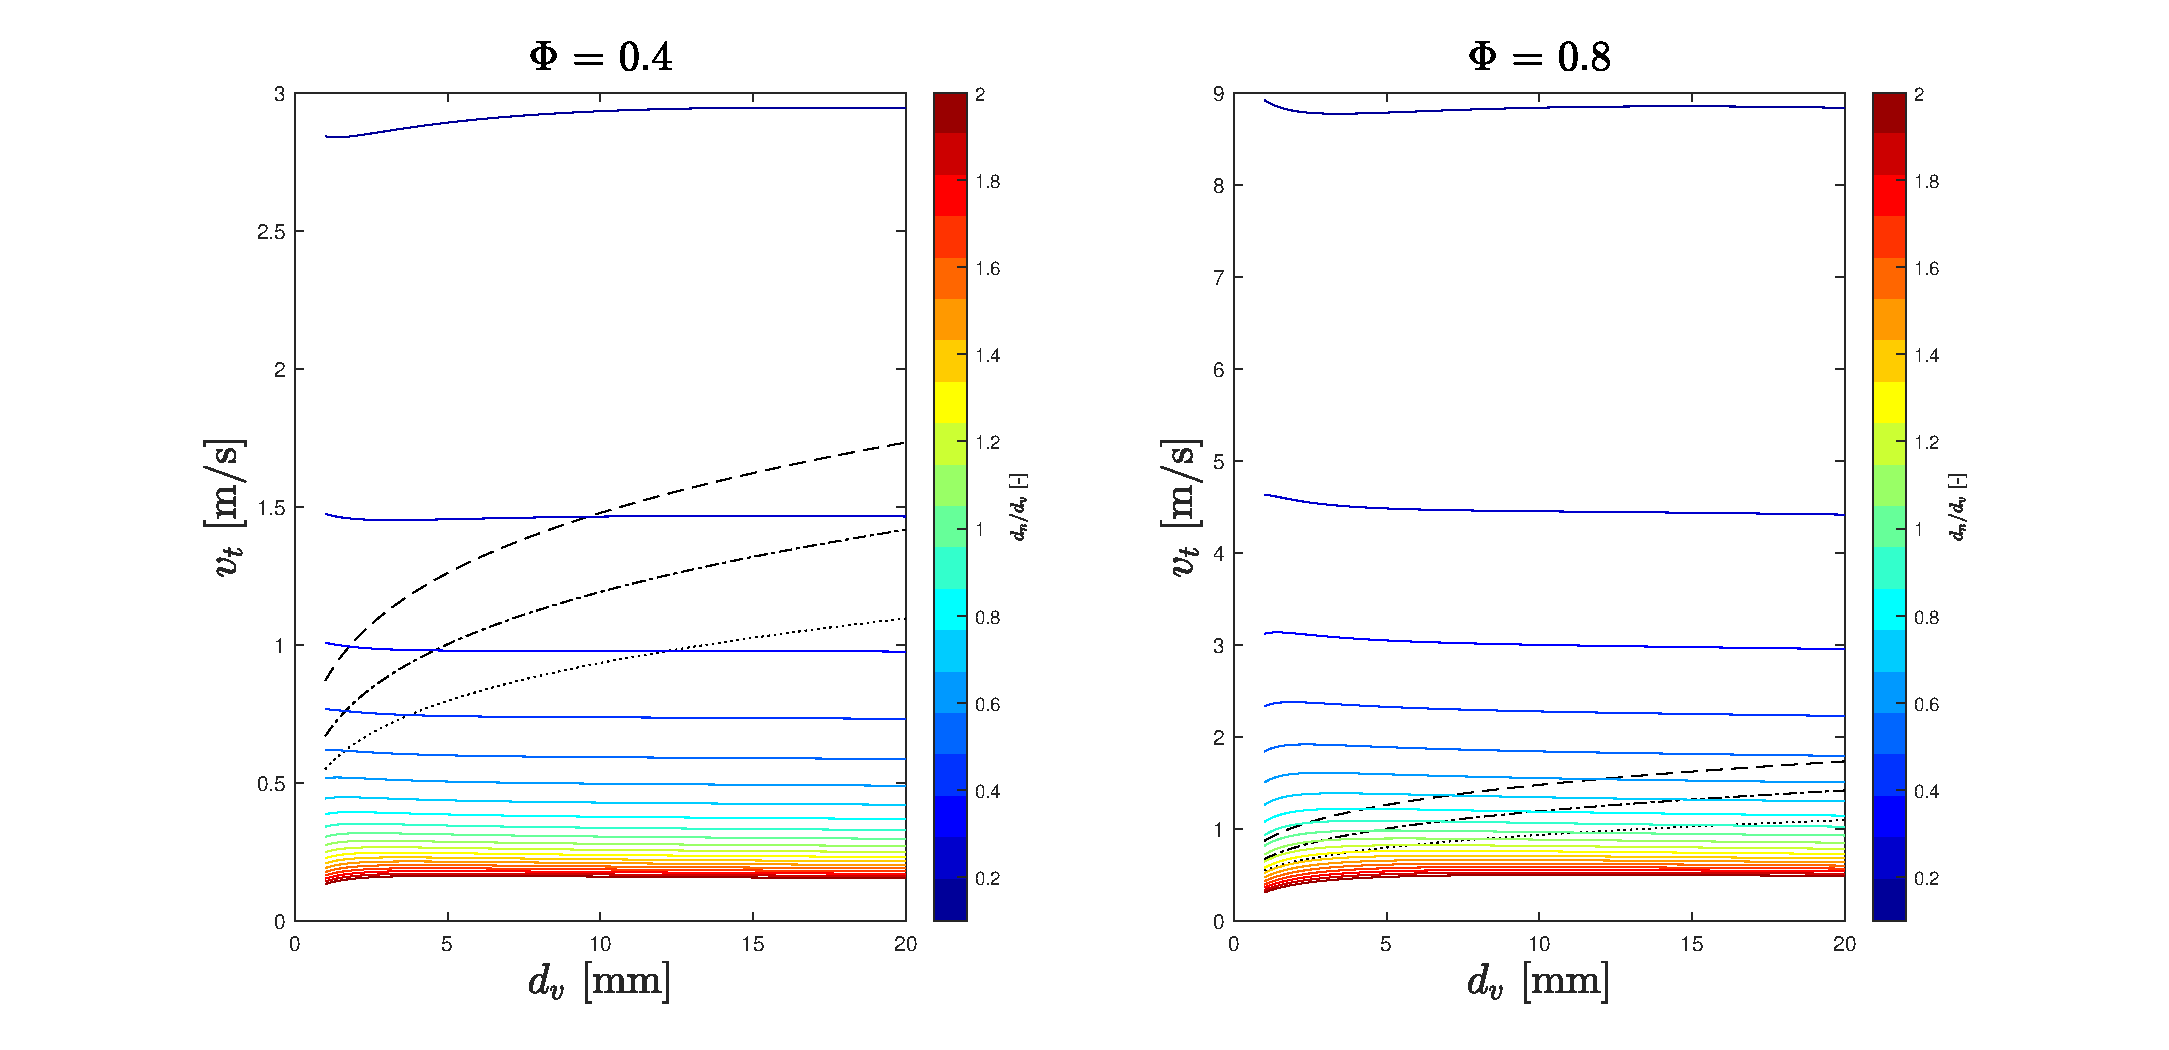
\includegraphics[width=\linewidth]{Ganser1.eps}
			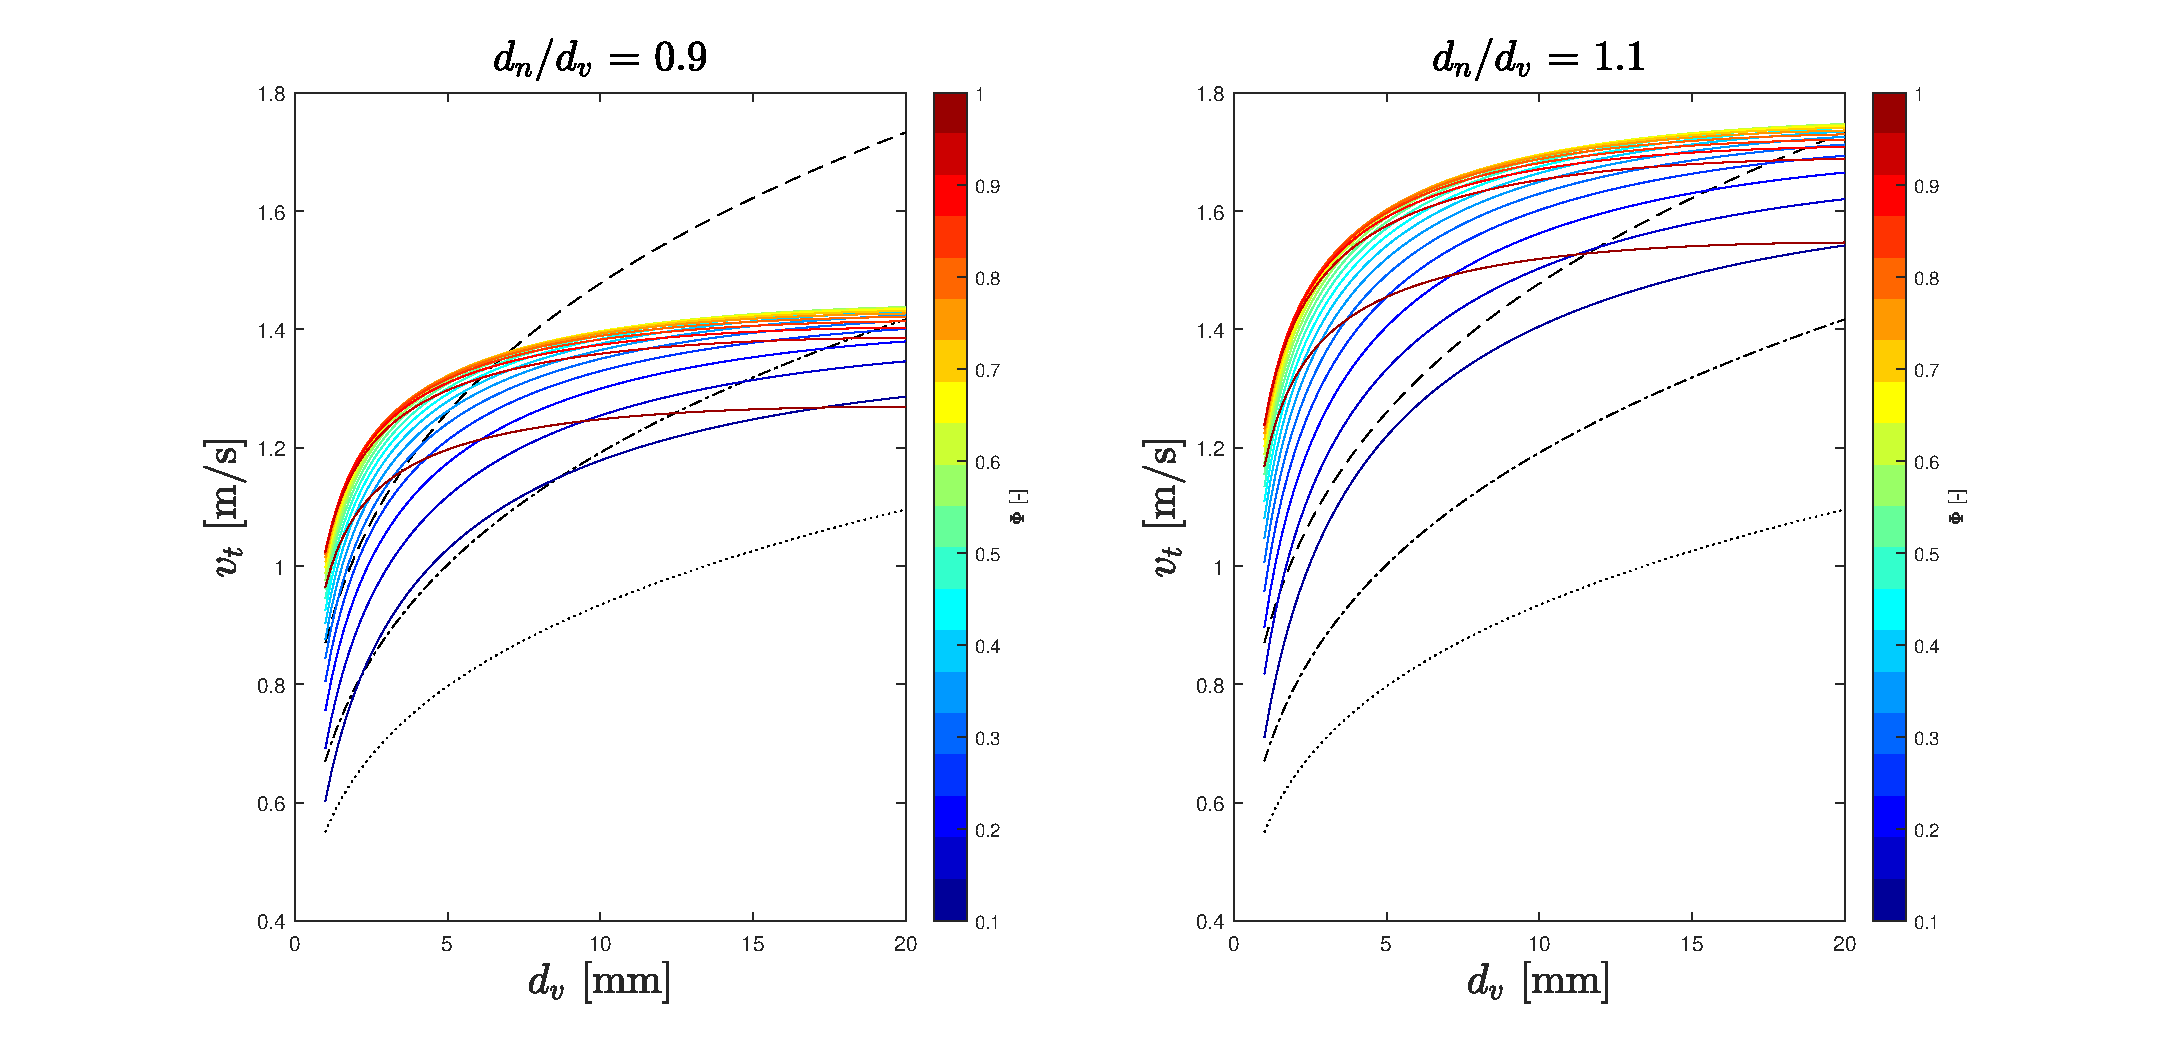
\includegraphics[width=\linewidth]{Ganser2.eps}
			\caption[Sensitivity study of the Ganser model.]{Sensitivity study of the Ganser model. Black lines are experimental curves from \cite{BrandesIkedEtAl-2008}, representing the mean terminal velocity of snowflakes during snowfalls of different temperatures: 
				$ \tikz[baseline] {\draw[dashed] (0,.5ex)--(.5,.5ex) ;} ~\SI{-1}{\celsius} $,
				$ \tikz[baseline] {\draw[dash dot] (0,.5ex)--(.5,.5ex) ;} ~\SI{-5}{\celsius} $,
				$ \tikz[baseline] {\draw[dotted] (0,.5ex)--(.5,.5ex) ;} ~\SI{-10}{\celsius} $}
			\label{fig: sensitivityGanser}
		\end{figure}	
		
		\begin{figure}
			\centering
			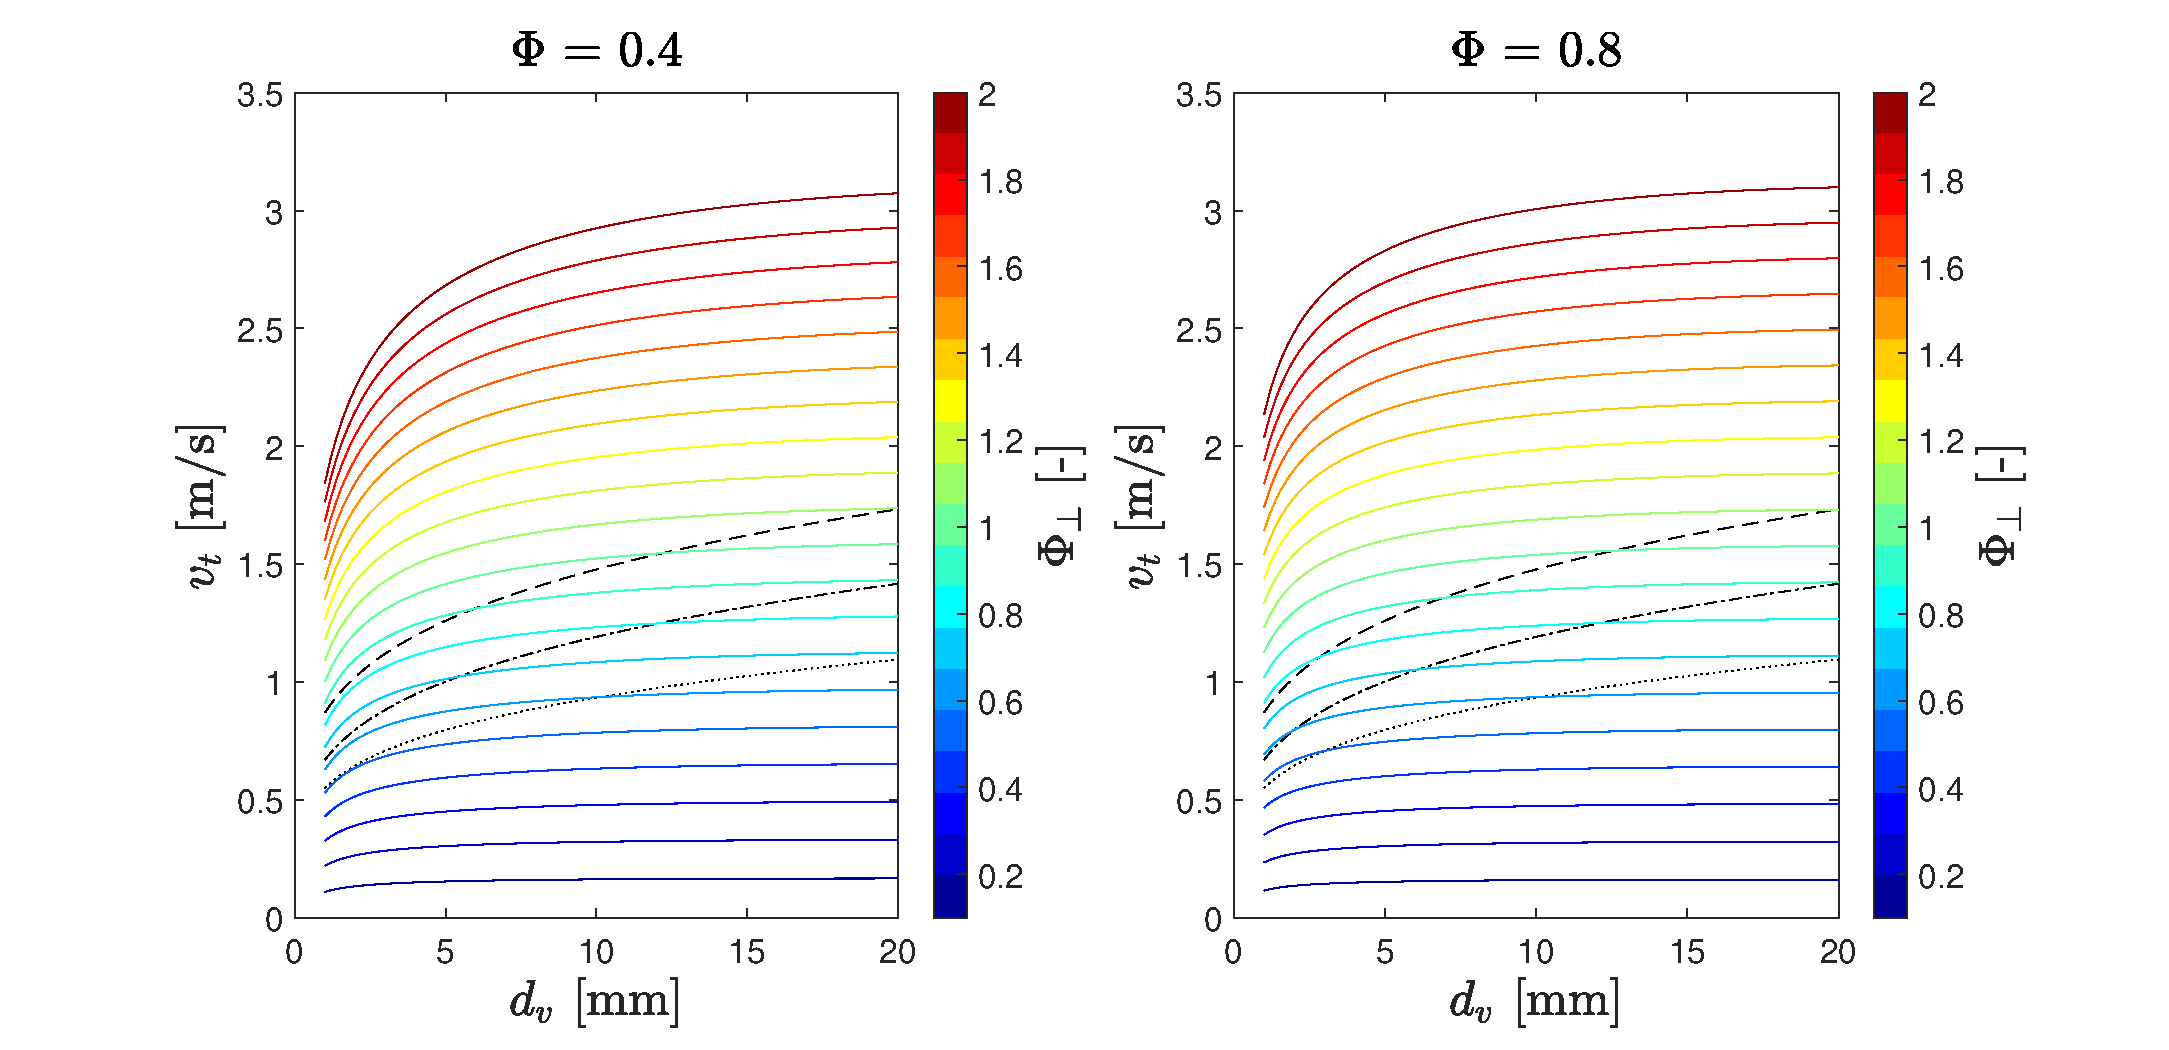
\includegraphics[width=\linewidth]{HS1.eps}
			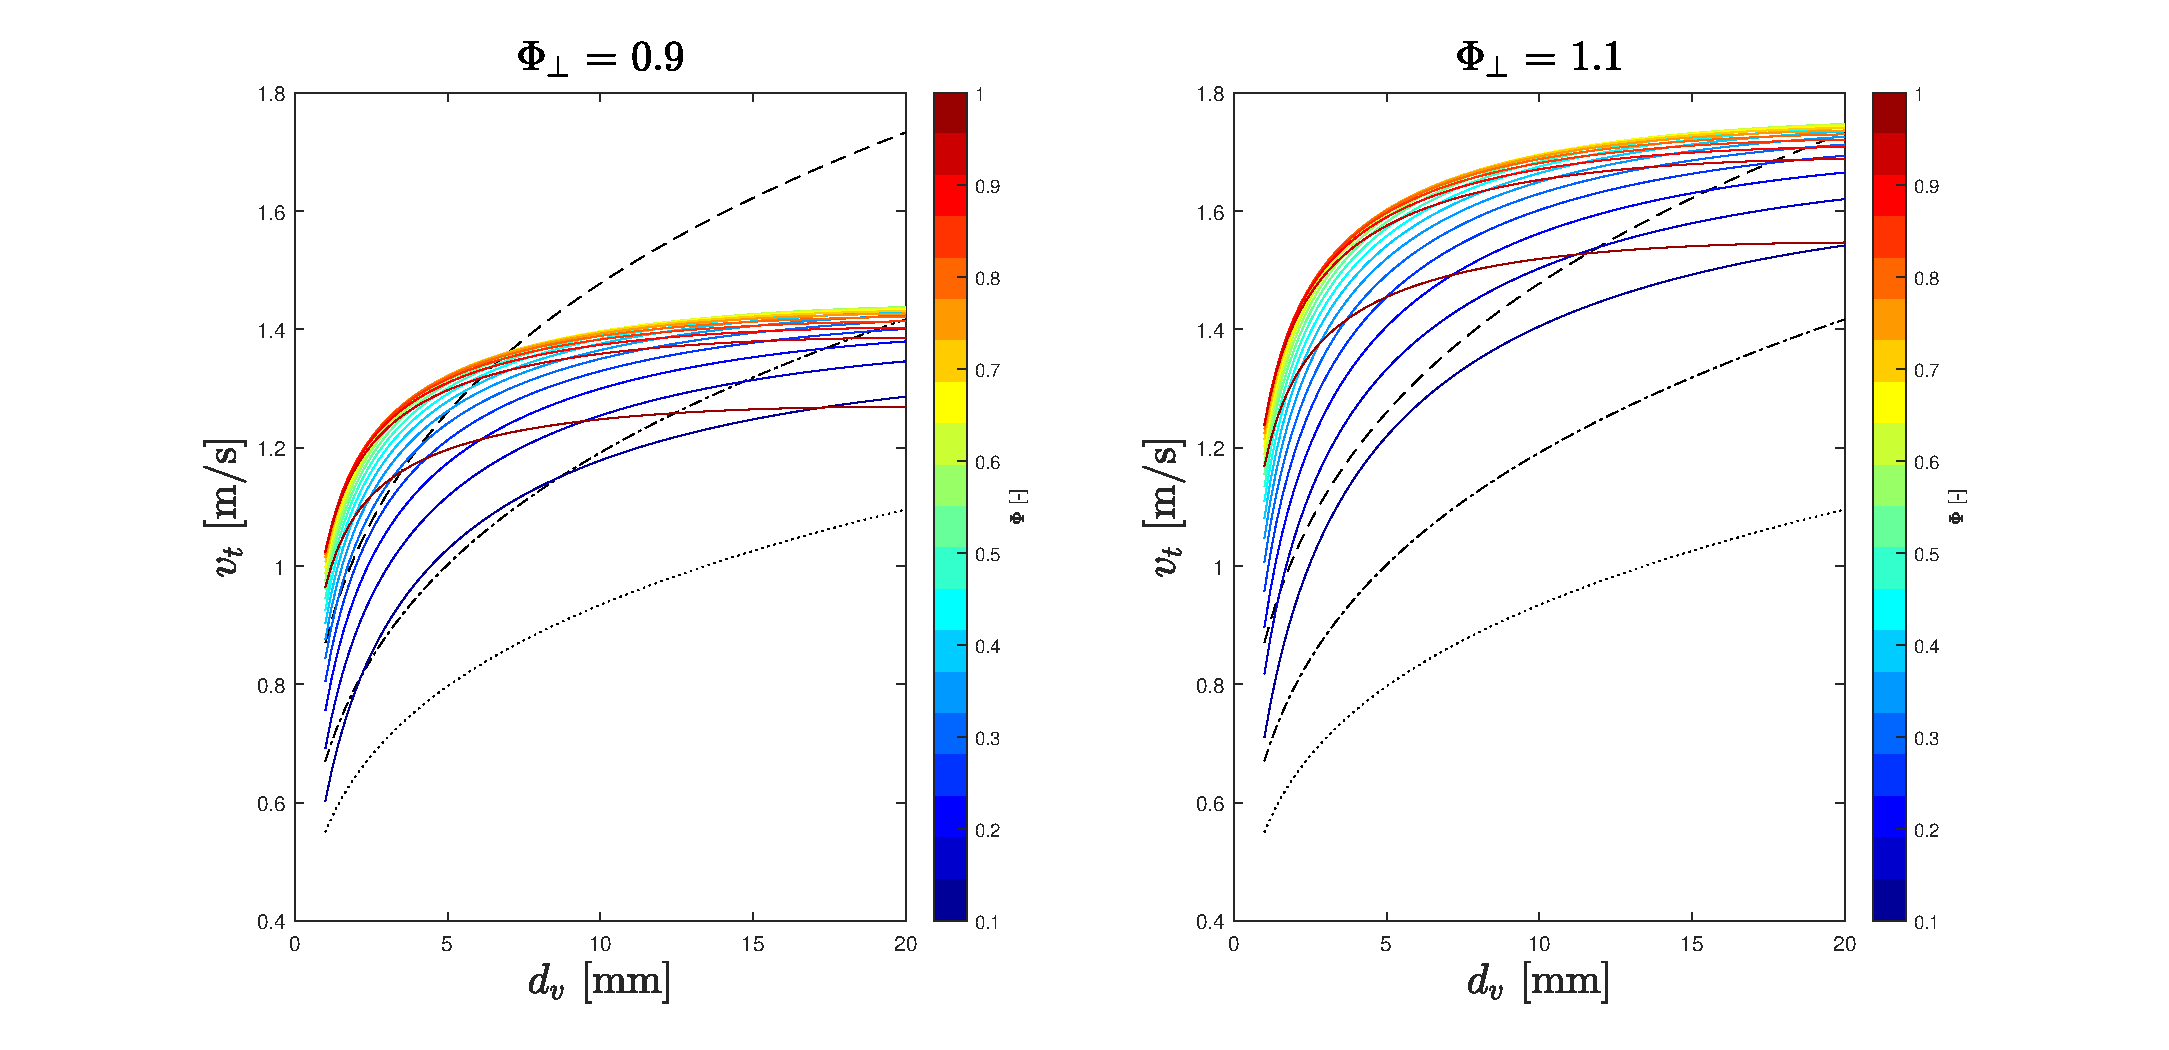
\includegraphics[width=\linewidth]{HS2.eps}
			\caption[Sensitivity study of the H\"oltzer and Sommerfeld model.]{Sensitivity study of the H\"oltzer and Sommerfeld model. Black lines are experimental curves from \cite{BrandesIkedEtAl-2008}, representing the mean terminal velocity of snowflakes during snowfalls of different temperatures: 
				$ \tikz[baseline] {\draw[dashed] (0,.7ex)--(.5,.7ex) ;} ~\SI{-1}{\celsius} $,
				$ \tikz[baseline] {\draw[dash dot] (0,.7ex)--(.5,.7ex) ;} ~\SI{-5}{\celsius} $,
				$ \tikz[baseline] {\draw[dotted] (0,.7ex)--(.5,.7ex) ;} ~\SI{-10}{\celsius} $}
			\label{fig: sensitivityHS}
		\end{figure}	
		
		The path we chose is to carry out a sensitivity study of the two models w.r.t. their free parameters (the shape descriptors), comparing them with the curves provided by Brandes \cite{BrandesIkedEtAl-2008}. These relations have on the abscissa the volume diameter of the particle and on the ordinate the mean terminal velocity of the snowflakes measured in their experimental campaigns. 
	
		For a more in-depth discussion on the calculation of the terminal velocity we refer the reader to the next section (\sref{sec: terminalVelocity}) and for the presentation of the Brandes' study to \sref{sec: Brandes}. 
	
		Some meaningful examples of this study are shown in \fref{fig: sensitivityGanser} and \fref{fig: sensitivityHS}. The top two figures represent curves obtained with fixed values of the first shape parameter ($ \Phi $), while the second shape parameter ($ \dn / \dv $ and $ \Phi_{\perp} $, respectively) is left free. The \textit{colorbar} on the right represents the value assumed by the free parameter. The range of values chosen and their discretization is the same for both models. We can observe an opposite behaviour of the obtained curves w.r.t. their second parameter, and, furthermore, that the Ganser model is more sensitive to a change in the ratio $ \dfrac{\dn}{\dv} $ than the model by H\"oltzer and Sommerfeld to a change in $ \Phi_{\perp} $. This appears clear recalling that $ \Phi_{\perp} \approx (\dfrac{\dv}{\dn})^2 $.
		Looking at the bottom figures, instead, we can observe a very similar behaviour of the two models w.r.t. a change in the sphericity.
		
		Both models appear to be a viable choice for the inference of the shape descriptors. We select the model by H\"oltzer and Sommerfeld arbitrarily, keeping in mind that its lesser sensitivity on $ \Phi_{\perp} $ will be helpful, as a minor precision on the inferred value of that parameter will be required.
		
		This choice is also supported by the recent study of the European project ICE GENESIS \red{can I cite them?}, which experimentally confirmed that the H\"oltzer and Sommerfeld model is the most appropriate for the description of snowflakes. 
		
%		comparison between the models and justification of my choice.
%		Comparison H\&S - Ganser: sensitivity study on the parameters of both models and why H\&S better suits the experimental curves of snow
%		
%		(+ "cite" the ICE GENESIS results proving that this model is the better one)		
		
	\section{Terminal Velocity calculation}
	\label{sec: terminalVelocity}
		The terminal velocity is the maximum velocity attainable by an object as it falls by effect of the gravity field. It is obtained, in the case of snow, when the sum of the drag ($ F_{D} $) and the buoyancy force ($ F_B $) balances the weight of the particle ($ W $). Under the assumption that the effects of aerodynamic forces and moments, on direction other than the falling one, are negligible, the governing equation reads:
		\begin{equation}
			\underbrace{\frac{1}{2} \rho v_t^2 S_{\perp} c_D(Re, \text{model}, \text{parameters})}_{F_{D}} = 
			\underbrace{\frac{\pi}{6} \dv^3 \rho_{\textup{p}} g}_{W} - 
			\underbrace{\frac{\pi}{6} \dv^3 \rho g}_{F_B}
			\label{eq: governing}
		\end{equation}
		which, after some simplification, can be written as:
		\begin{equation}
			\vt^2 c_D(Re(\vt, \dv), \text{model}, \text{parameters}) = 
			\frac{\pi}{3} \dfrac{\rho_{\textup{p}(\dv)} - \rho}{\rho} \dfrac{\dv^3}{S_{\perp}} g
			\label{eq: terminalVelocity}
		\end{equation}
		The reference surface is taken as the area of the particle projected to a plane perpendicular to the velocity vector and can be retrieved from the shape descriptor if the model accounts for the orientation of the particle; it is taken as $ \pi \dv^2 $ otherwise. Equations \ref{eq: areaGanser} and \ref{eq: areaHS} give the specialization of the reference surface for the Ganser and the H\"oltzer and Sommerfeld models, respectively.
		\begin{multicols}{2}
			\begin{equation}
				S_{\perp} = \pi \dn^2 = \pi \left( \frac{\dn}{\dv} \right)^2 \dv^2
				\label{eq: areaGanser}
			\end{equation}\break
			\begin{equation}
				S_{\perp} \simeq A_{\textup{p}, \perp} = \dfrac{\pi}{4 \Phi}
				\label{eq: areaHS}
			\end{equation}
		\end{multicols}
		
		For the calculation of $ \rho_{\textup{p}} $, an empirical formula found by Brandes \cite{Brandes-2008} is used:
		\begin{equation}
			\rho_{\textup{p}(\dv)} = 0.178\ \dv^{-0.922}
		\end{equation}
		where the density of snow is measured in $ kg / m^3 $ and the diameter is measured in $ m $. 
		The equation for the terminal velocity (\ref{eq: terminalVelocity}) is thus solved iteratively for the unknown $ \vt $, while $ \dv $ is the independent variable, and \textit{model} and \textit{shape} are the free parameters coming from the shape descriptors.
		
%		Equation for the terminal velocity of a particle: how to calculate every term starting from the diameter and the shape parameters
	
